\documentclass[final,1p,times,authoryear,12pt]{elsarticle}

%% The amssymb package provides various useful mathematical symbols
\usepackage{amssymb}
%% The amsthm package provides extended theorem environments
%% \usepackage{amsthm}

\usepackage{longtable}
\usepackage{paralist}
\usepackage{booktabs}
\usepackage{float}
\restylefloat{table}
\usepackage{graphicx}
\usepackage{subcaption}
\usepackage{hyperref}
%\usepackage{geometry}
\usepackage{pdflscape}
\usepackage{color}
\usepackage{xcolor} 
\usepackage{xspace}
\usepackage{fullpage}
\usepackage{tabularx}
\usepackage{wrapfig}
\providecommand{\wss}[1]{\textcolor{blue}{\textit{#1}}}

\begin{document}
\begin{frontmatter}

\title{State of the Practice for Open-Source Neural Network Software}
\address{Department of Computing and Software \\
McMaster University \\
Hamilton, Ontario, Canada}

\begin{abstract}
% \wss{150--250 word abstract: problem/gap, method (measurement template + repo metrics + AHP),
%  headline results, contributions (DomainX tool + dataset + findings). 
%  one-line pointer to the DomainX repo and a brief data availability statement.}

Open-source neural network (NN) software plays an important
role in modern AI research and development. Assessing the
software-engineering practices of NN packages, however, is
challenging because relevant evidence is distributed across
public artifacts such as documentation, tests, issue trackers,
releases, and continuous integration (CI) configurations.

This paper presents DomainX, a tool-supported workflow for
conducting a state-of-practice assessment of open-source NN
software based on a published methodology. DomainX supports
evidence capture, scoring through a measurement template
spanning nine software-quality attributes, incorporation of
repository-based measures, and overall comparison using the
Analytic Hierarchy Process (AHP).

We apply this workflow to a curated shortlist of 28
open-source NN software packages and produce a traceable
dataset containing template responses, repository-based
measures, and package-level references (project website and
repository URLs). \textbf{[RESULTS SUMMARY TO BE ADDED AFTER 
FINAL RANKING IS CONFIRMED.]}
A companion repository provides the DomainX tool and
associated assessment artifacts to support review and reuse.
\end{abstract}

\begin{keyword}
% \wss{state of practice; research software; NLP libraries; software quality;
%  measurement template; AHP; reproducibility; traceability.}
state of practice; research software; neural network libraries; software quality;
measurement template; Analytic Hierarchy Process (AHP); traceability; reproducibility; repository mining.
\end{keyword}

\end{frontmatter}

%%%%%%%%%%%%%%%%%%%%%%%%%%%%%%%%%%%%%%%%%%
%%%%%%%%%%%%%%%%%%%%%%%%%%%%%%%%%%%%%%%%%%
\section{Introduction}\label{introduction}
%%%%%%%%%%%%%%%%%%%%%%%%%%%%%%%%%%%%%%%%%%
%%%%%%%%%%%%%%%%%%%%%%%%%%%%%%%%%%%%%%%%%%
% \wss{why software quality matters for research/engineering outcomes 
% and why a state-of-practice assessment is useful for the domain.
%   why assessment is difficult in practice (evidence scattered across docs/tests/issues/CI,
%    manual spreadsheet workflows are time-consuming and hard to audit/reproduce).}

% \wss{State contributions explicitly as a short bullet list: DomainX tool support (include repo pointer), ffinal shortlist + completed dataset,
%  ranking + sensitivity analysis + insights/recommendations.}

% \wss{ short paragraph that states what software is being evaluated: 
% the set of open-source packages in the selected domain, what they generally do, the final shortlist size,
%  and a pointer to the appendix/table listing the packages.}

% \wss{ roadmap of the remainder of the paper.}

Research and engineering outcomes increasingly depend on
software, and the quality of that software affects
reliability, maintainability, and reproducibility. In domains
where open-source libraries are widely reused, understanding
current development practice is an important step toward
improving it. A \emph{state-of-practice} assessment provides
a structured way to characterize what developers commonly do
in a domain by evaluating representative software packages
against explicit software-quality criteria using traceable
evidence.

Conducting such assessments rigorously is challenging in
practice. Evidence relevant to software quality is
distributed across many public artifacts, including
documentation, tutorials, repository history, tests, issue
trackers, releases, and continuous integration (CI)
configurations. This makes the assessment process
time-consuming and creates challenges for auditability,
maintenance, and reproducibility as repositories evolve over
time.

This paper presents a tool-supported state-of-practice assessment for \emph{neural network (NN) software}. 
The target audience is developers and maintainers of NN software; accordingly, the scope is restricted to NN packages rather than 
general-purpose NN-supporting libraries from adjacent communities. The assessment workflow follows a published state-of-practice 
methodology based on (i) a measurement template organized by software-quality attributes, (ii) repository-based measures extracted 
from public repositories, and (iii) an Analytic Hierarchy Process (AHP) ranking procedure to combine evidence into transparent 
comparisons.

The contributions of this work are:
\begin{itemize}
  \item A curated shortlist of 28 open-source NN software packages evaluated using a consistent, evidence-based procedure (Appendix~\ref{app-packages}).
  \item A traceable assessment dataset recording measurement-template responses, repository-based measures, and package-level references (project website and repository
        URLs) for auditability and reuse.
  \item DomainX, a tool that supports evidence capture, scoring, ranking computations, and export of results to reduce manual effort and improve traceability (\url{https://github.com/thaafei/DomainX}).
\end{itemize}

The remainder of this paper defines key concepts and summarizes background (Section~\ref{background}), describes the assessment methodology and tool support (Section~\ref{methods}), 
and reports results and observations from applying the approach to the shortlisted packages (Section~\ref{results}).
 The paper concludes with discussion, recommendations, and limitations (Sections~\ref{discussion}--\ref{conclusion}).

%%%%%%%%%%%%%%%%%%%%%%%%%%%%%%%%%%%%%%
%%%%%%%%%%%%%%%%%%%%%%%%%%%%%%%%%%%%%%
\section{Background and Definitions} \label{background}
%%%%%%%%%%%%%%%%%%%%%%%%%%%%%%%%%%%%%%
%%%%%%%%%%%%%%%%%%%%%%%%%%%%%%%%%%%%%%
% \wss{Define key terms: research software, domain, library/package,
%  and evidence (public artifacts such as docs, repository history, issues, tests, CI configs).
%    state-of-the-art vs state-of-practice and why gaps occur.}

% \wss{brief overview of the assessment methodology being followed (cite the methodology paper)
%  and  short explanation of AHP and why it is used for ranking in this context.}
%%CITE THE METHODOLOGY PAPERRR

In this paper, \emph{research software} refers to software used to support scientific or engineering work such as data processing,
 model training or inference, experimentation, and analysis. A \emph{domain} is a coherent problem area characterized by 
 shared goals and typical workflows; in a state-of-practice assessment, the domain determines which software packages are 
 relevant and what evidence is meaningful for evaluation. A \emph{library} (or package) is a reusable software component intended
  to be integrated into other programs. We use \emph{evidence} to mean publicly available artifacts that indicate software-development
   practice, including documentation and tutorials, repository history (commits and releases), issue trackers and pull requests,
    tests, and continuous integration (CI) configurations.

The \emph{state of the art} describes the most advanced methods and recommended best practices reported in research and practitioner
 literature. The \emph{state of practice} describes what is commonly done in real projects: the tools used, the artifacts produced,
  and the quality-related practices that are routinely applied. Gaps between state of the art and state of practice are common,
   particularly in research settings where incentives and timelines may prioritize functionality and 
   novelty over long-term maintainability, transparency, or reproducibility. 
   A state-of-practice assessment aims to characterize this reality using explicit criteria and traceable evidence,
    enabling systematic comparison and targeted recommendations.

A published state-of-practice methodology guides our
assessment by combining (i) a measurement template grounded
in software-quality attributes with (ii) evidence extracted
from public artifacts and repository-based measures,
enabling comparisons that are intended to be reproducible
and auditable \cite{MethodologyPaper}.

To produce an overall comparison across multiple criteria, we use the Analytic Hierarchy Process (AHP), 
a multi-criteria decision-making method that derives weights from pairwise comparisons of criteria and aggregates scores accordingly. 
AHP is well suited to this setting because it makes weighting assumptions explicit and supports transparent trade-offs
 among software-quality attributes. In this work, AHP is used to compute an evidence-based ranking and to support sensitivity analysis
  on how rankings change under different weighting choices.
 %%%%%%%%%%%%%%%%%%%%%%%%%%%%%%%%%%%%%%
%%%%%%%%%%%%%%%%%%%%%%%%%%%%%%%%%%%%%%
\section{Methods}\label{methods}
%%%%%%%%%%%%%%%%%%%%%%%%%%%%%%%%%%%%%%
%%%%%%%%%%%%%%%%%%%%%%%%%%%%%%%%%%%%%%

\subsection{Domain framing and scope}\label{scope}
% \wss{Define the assessed domain, what is in scope vs out of scope for “NN software” in this assessment. 
% Include inclusion/exclusion criteria (public repo, docs, relevant functionality, examples).}

Neural network (NN) software is defined here as open-source libraries whose primary purpose is to enable the development, 
training, deployment, analysis, or direct use of neural network models. The target audience for this assessment is developers
 and maintainers of NN software. Accordingly, general-purpose NN-supporting packages
 (e.g., numerical computing, data manipulation, or plotting libraries) are out of scope because they belong to different developer 
 communities and would confound interpretation of NN software development practice. 
 Packages are included when they have a publicly accessible repository and sufficient publicly available artifacts 
 (e.g., documentation and repository history) to support evidence-based evaluation.

\subsection{Candidate identification and filtering}\label{filtering}
% \wss{Describe how candidates were identified (sources/search style) , how filtering produced the final set.
%  Report counts at each step and the final shortlist size. Final shortlist: 28. 
%  Point to Appendix~\ref{app-packages} for the full list and exclusions (see emails).}

 Candidate packages were compiled by aggregating package names from authoritative sources and normalizing duplicates 
 and naming variants. To align the assessment with the intended audience, packages that were NN-supporting rather than NN software 
 were removed. Following supervisor guidance, NN software packages were retained even when they appeared only once across the
  authoritative sources to prioritize completeness of coverage. The final shortlist contains 28 packages. 
  The full shortlist and excluded candidates (with brief reasons) are provided in Appendix~\ref{app-packages}.

\subsection{Evidence sources and data collection}\label{data}
% \wss{Describe evidence sources used to score each package: 
% documentation/README, tutorials/examples, repository history, releases, issues/PRs, tests, CI/CD configuration. 
%  automated extraction vs manual inspection (repo metrics vs others). 
%   how evidence was recorded to make results traceable and auditable? (metrics spreadsheet)}

Evidence was derived from publicly available artifacts associated with each package, 
including documentation (e.g., README and installation guides), tutorials/examples, 
repository history, releases, issue trackers and pull requests, tests, and continuous integration (CI) configuration when available. 
Repository-based measures were extracted using automated scripts/tools. Some measurement-template questions required manual
 judgment (e.g., installation and usage guidance, presence of tests, or CI configuration). 
 Responses were recorded directly in the measurement template, and each package entry includes a project website URL and a source-code 
 repository URL that can be used to verify the recorded responses against the corresponding public artifacts.

\subsection{Measurement template and scoring}\label{template}
% \wss{the assessment uses the methodology paper’s measurement template organized by software qualities. 
% Qualities assessed: installability, correctness \& verifiability, surface reliability, surface robustness, surface usability, 
% maintainability, reusability, surface understandability, visibility/transparency. 
%  scoring approach summary (evidence $\rightarrow$ question response $\rightarrow$ normalized score $\rightarrow$ aggregation). 
%   rules for missing/unclear evidence and any consistency checks.}

The assessment uses a published measurement template organized by software-quality attributes. 
The qualities assessed are: installability; correctness and verifiability; surface reliability; surface robustness; surface usability;
 maintainability; reusability; surface understandability; and visibility/transparency. 
 For each package, publicly available evidence was used to answer template questions and derive per-quality scores according 
 to the template’s scoring rules. Scores were normalized and aggregated to support cross-package comparison.
  When evidence was missing or ambiguous, responses were recorded conservatively and flagged for traceability.

\subsection{Repository-based measures}\label{metrics}
% \wss{Describe repository/empirical measures collected (e.g. GitHub-based measures + codebase statistics). 
%  the tools/sources used (e.g., GitHub API, scc, git\_stats) and what each category captures. 
%   enough detail to reproduce extraction.}

Repository-based measures complement the measurement template
by capturing observable project characteristics and
development activity from public repositories. Using the same
repository-measure framework defined in the methodology
paper, the collected raw data includes GitHub-derived
measures such as stars, forks, watchers, open and closed
pull requests, and open and closed issues, together with
repository statistics such as number of developers,
programming languages, file counts, lines of code, comment
lines, blank lines, binary files, total commits, and commit
activity over recent yearly and monthly intervals
\cite{MethodologyPaper}. The methodology identifies
\texttt{git\_stats} and \texttt{scc} as the tools used to
collect repository statistics, with GitHub repository data
used when the project is hosted on GitHub
\cite{MethodologyPaper}.

In addition to raw measures, the methodology defines a small
set of processed measures derived from the raw data. These
include project status (alive or dead), percentage of issues
closed, and percentage of code that is comments
\cite{MethodologyPaper}. Together, these measures provide
additional context for interpreting the quality scores
recorded in the measurement template.

\subsection{Ranking method (AHP) and sensitivity analysis}\label{ahp}
% \wss{Explain how AHP was used to compute weights and produce an overall ranking from quality scores. 
% Describe how pairwise comparisons were obtained and how final scores were computed. 
%  sensitivity analysis results (plan if not yet complete) to assess ranking stability under reasonable weight changes. 
%  ranking supports comparison/insight rather than a universal claim of “best.”}
To produce an overall comparison across multiple quality
criteria, this work uses the Analytic Hierarchy Process
(AHP), following the methodology paper
\cite{MethodologyPaper}. AHP is a multi-criteria
decision-making technique based on pairwise comparisons. In
this context, it is used to compare software packages using
the quality scores derived from the measurement template.
The pairwise comparisons are used to construct matrices that
yield an overall score for each package under the selected
criteria weights \cite{MethodologyPaper}.

As emphasized in the methodology, the ranking is not meant
to identify a single universally ``best'' package. Instead,
it is intended to provide insight into the top-performing
set of packages and to support interpretation of domain-wide
patterns \cite{MethodologyPaper}. The methodology also
includes sensitivity analysis so that the stability of the
ranking can be examined under uncertainty or variation in
the quality scores and weighting choices \cite{MethodologyPaper}.


\subsection{Tool support: DomainX}\label{domainx}
% \wss{ DomainX at the key-feature level: centralized evidence capture, structured template completion, 
% metric extraction, AHP computation, and export of results.  reduced manual effort and improved traceability/auditability. 
% Repository: \url{https://github.com/thaafei/DomainX} }
DomainX supports a tool-based workflow for conducting the
assessment and managing the resulting dataset. It provides an
interactive interface for recording measurement-template
responses and repository-based measures across the shortlisted
packages. DomainX also integrates the Analytic Hierarchy
Process (AHP) computation used to aggregate quality-level
scores into an overall comparison and visualizes the resulting
ranking. In addition, the tool supports export of assessment
artifacts for reporting and review. The DomainX implementation
is available at \url{https://github.com/thaafei/DomainX}.

\begin{figure}[H]
  \centering
  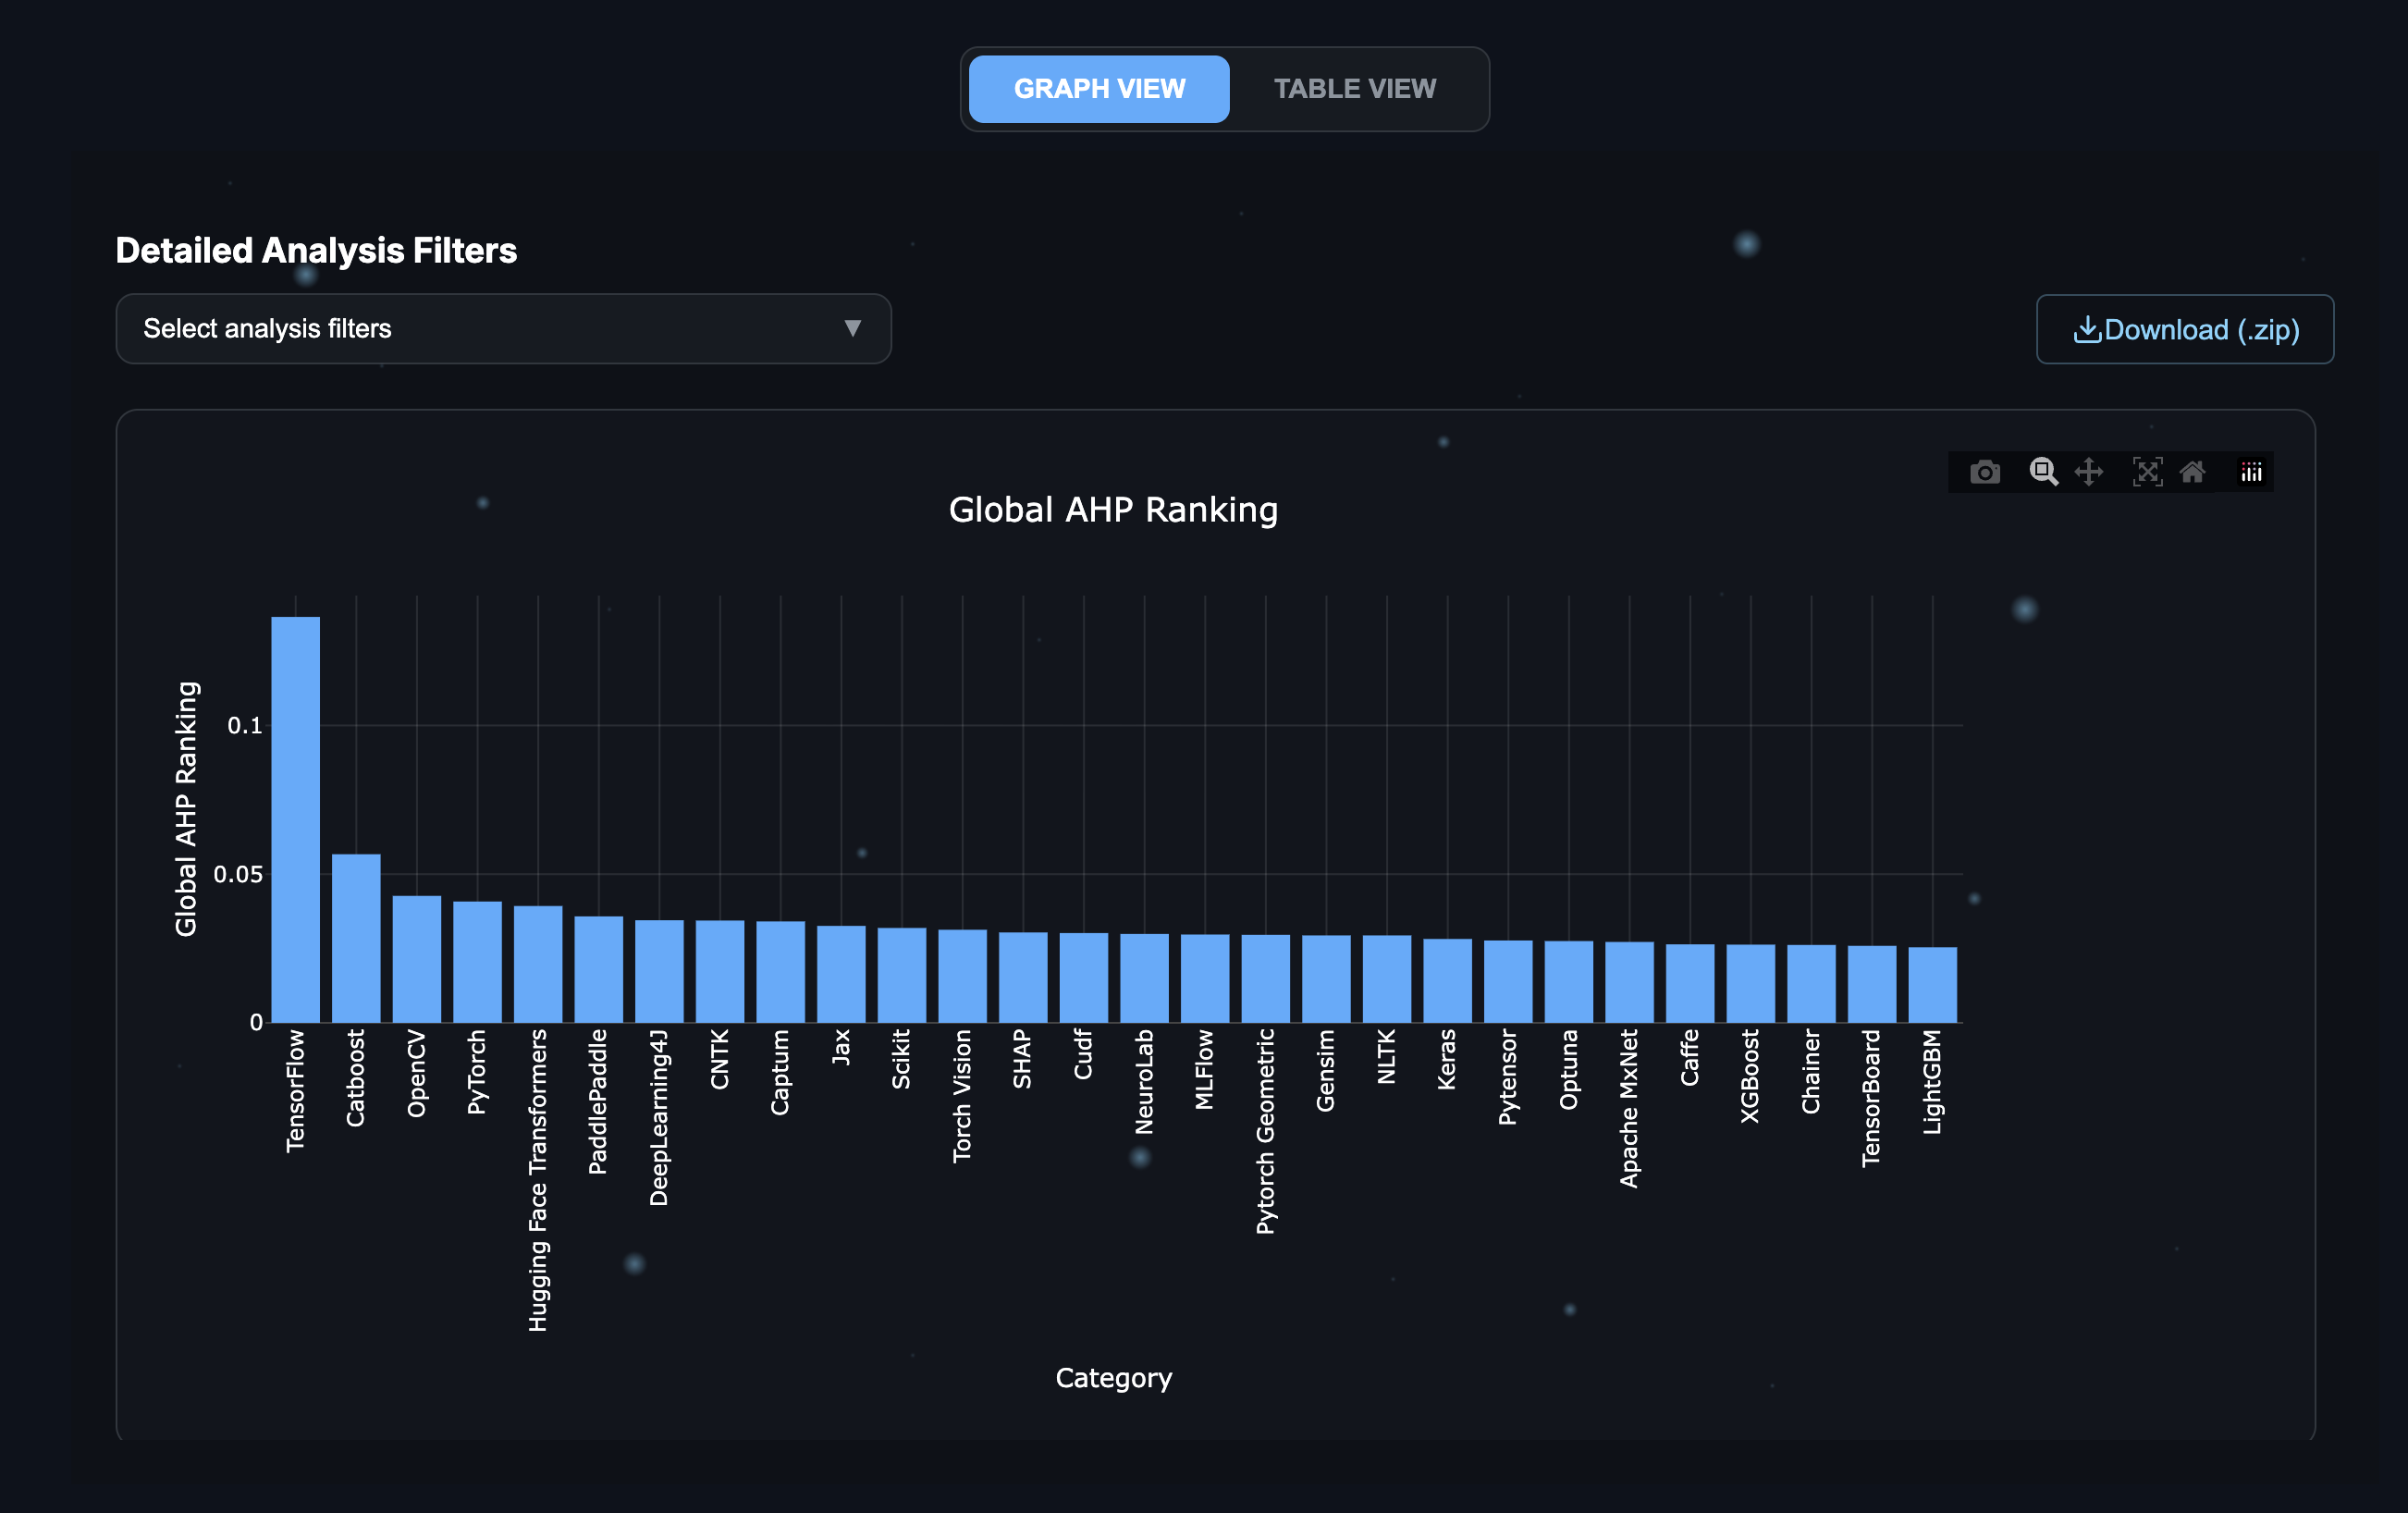
\includegraphics[width=\textwidth]{snapshots/domainxgraphview.png}
  \caption{DomainX graph view illustrating the overall AHP
ranking for the assessed packages.}
  \label{fig:domainx}
\end{figure}
%%add snapshot

\subsection{Environment and reproducibility}\label{env}
% \wss{Describe the evaluation environment and  steps to take for reproducing (e.g. pinned versions, standardized install attempts). 
% Mention Dockerfiles used for older packages where needed and connect this to repeatability and transparency.}

Following the methodology, installation-based assessment is
performed in a clean, isolated environment so that software
packages are evaluated on a more level playing field
\cite{MethodologyPaper}. The methodology recommends using
virtual machines (VMs) because they provide a fresh
environment for each installation attempt, reduce conflicts
with pre-existing libraries, and help avoid
``works-on-my-computer'' effects \cite{MethodologyPaper}.

In the methodology, repository-based data is collected first,
followed by installation and measurement-template scoring.
The methodology also recommends recording environment details
for each installation context, including the operating system
and virtualization environment, to support repeatability
\cite{MethodologyPaper}. In the present work, some older packages required additional environment setup
because their dependencies and installation requirements were
not readily compatible with a modern default environment. In
these cases, containerized environments defined through
Dockerfiles were used to reproduce a more suitable setup and
improve consistency across installation attempts. These choices
were made to improve consistency and transparency of the
assessment process.

%%%%%%%%%%%%%%%%%%%%%%%%%%%%%%%%%%%%%%
%%%%%%%%%%%%%%%%%%%%%%%%%%%%%%%%%%%%%%
\section{Results}\label{results}
%%%%%%%%%%%%%%%%%%%%%%%%%%%%%%%%%%%%%%
%%%%%%%%%%%%%%%%%%%%%%%%%%%%%%%%%%%%%%

\subsection{Descriptive summary of assessed packages}\label{results-summary}
% \wss{Summarize the evaluated set (final no., alive/dead counts, languages/activity/licensing if reported). 
% Present  statistics that help give insight into the domain landscape before ranking.}

The final shortlist contains 28 open-source neural network
software packages selected according to the scope and
filtering process described in Section~\ref{methods}. Based
on the project-status information recorded in the assessment
template, 23 packages were classified as alive and 5 were
classified as dead. This mix of active and inactive projects
provides important context for interpreting the assessment
results, since project activity can affect the availability
of documentation, testing artifacts, maintenance signals,
and other observable evidence of development practice.

\subsection{Overall ranking}\label{results-ranking}
% \wss{ the final ranking table and a short explanation of how to read it. 
% Highlight  top-ranked packages without overconfidence/ overdoing it. Reference DomainX ranking output as a figure/table.}
\subsection{Overall ranking}\label{results-ranking}

\subsection{Overall ranking}\label{results-ranking}

Figure~\ref{fig:overall-ranking} presents the overall AHP
ranking for the shortlisted packages as produced by
DomainX. TensorFlow achieved the highest overall score
(13.65\%), followed by Catboost (5.67\%), OpenCV
(4.27\%), PyTorch (4.08\%), and Hugging Face
Transformers (3.93\%). At the lower end of the ranking,
LightGBM (2.54\%), TensorBoard (2.59\%), Chainer
(2.62\%), XGBoost (2.63\%), and Caffe (2.64\%) obtained
the smallest overall scores.

A notable feature of the ranking is the large gap between
TensorFlow and the rest of the shortlisted packages.
Beyond the top-ranked package, many libraries are clustered
within a comparatively narrow score range, suggesting that
the middle and lower portions of the ranking are more
densely packed. Under the current configuration, many
category-level scores are identical across packages, so
differences in the overall ranking are driven primarily by
variation in installability, correctness and
verifiability, and repository-based measures.

\begin{figure}[H]
  \centering
  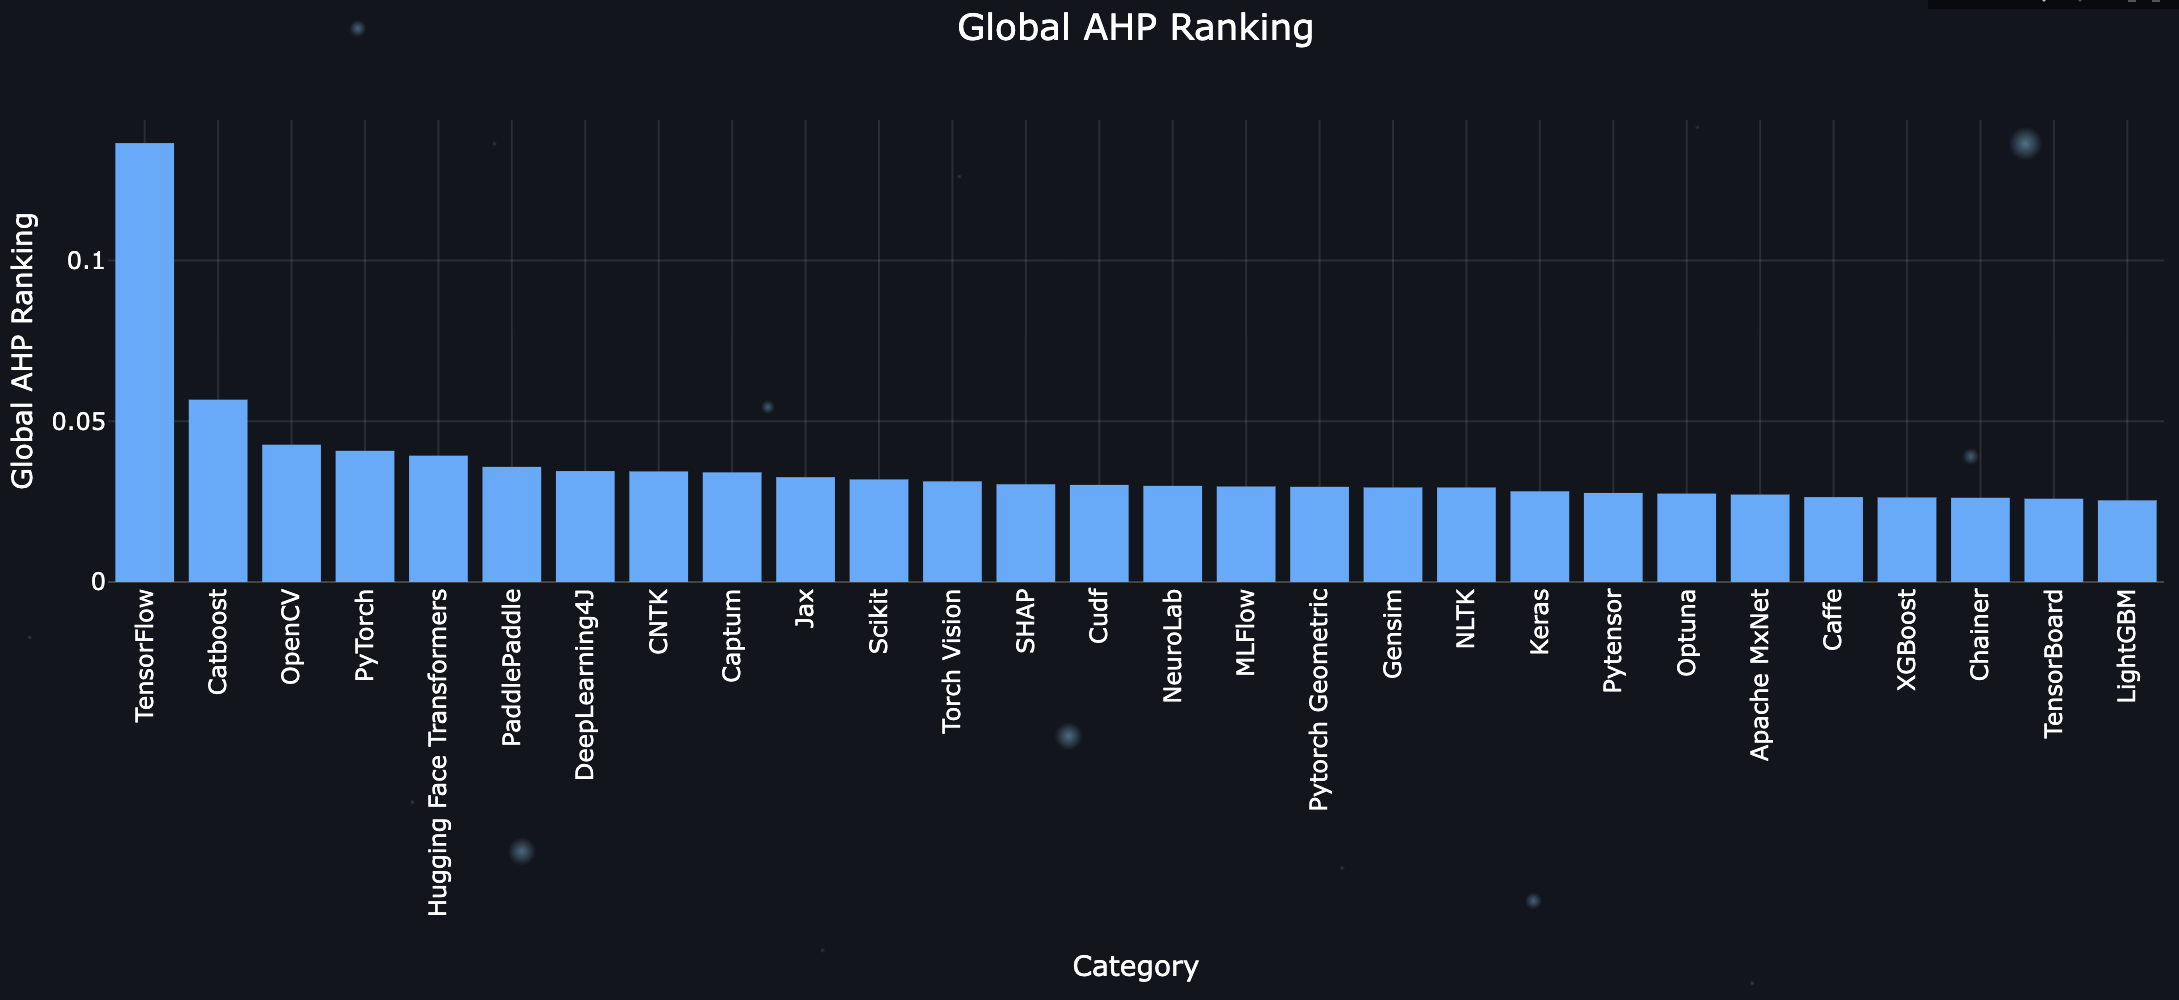
\includegraphics[width=\textwidth]{snapshots/graphview.png}
  \caption{Overall AHP ranking for the shortlisted packages
  as visualized in DomainX.}
  \label{fig:overall-ranking}
\end{figure}

\begin{table}[H]
\centering
\caption{Top 10 packages by overall AHP score.}
\label{tab:top10-ranking}
\begin{tabular}{r l r}
\toprule
\textbf{Rank} & \textbf{Package} & \textbf{Overall Score} \\
\midrule
1  & TensorFlow                & 13.65\% \\
2  & Catboost                  & 5.67\%  \\
3  & OpenCV                    & 4.27\%  \\
4  & PyTorch                   & 4.08\%  \\
5  & Hugging Face Transformers & 3.93\%  \\
6  & PaddlePaddle              & 3.58\%  \\
7  & DeepLearning4J            & 3.45\%  \\
8  & CNTK                      & 3.44\%  \\
9  & Captum                    & 3.41\%  \\
10 & Jax                       & 3.26\%  \\
\bottomrule
\end{tabular}
\end{table}

Table~\ref{tab:top10-ranking} lists the top 10 packages
under the current overall AHP ranking. TensorFlow is the
clear top-ranked package, while the remaining top 10
packages are more tightly clustered.

\subsection{Quality-by-quality breakdown}\label{results-byquality}
% \wss{ results by quality attribute (tables/figures). Identify strong/weak packages per quality and report domain-wide patterns
%  supported by evidence.}
Figure~\ref{fig:quality-heatmap} summarizes the per-quality
results across the 28 shortlisted packages. The heatmap
shows that several assessed categories take nearly the same
value across most of the shortlisted packages. In
particular, surface reliability, surface robustness,
surface usability, reusability, visibility/transparency,
and surface understandability are highly uniform in the
current results. As a result, the most visible differences
across packages arise in installability, quality, and
correctness and verifiability.

Correctness and verifiability has the strongest visible
effect on the ranking. TensorFlow obtains the highest value
in this category (99.98\%), substantially exceeding the
other shortlisted packages, and this contributes strongly to
its position as the top-ranked package overall.

Installability also differentiates several packages.
Catboost records the highest installability value
(18.18\%), followed by Captum (11.36\%) and a group of
packages including DeepLearning4J, NeuroLab, OpenCV, and
TorchVision (6.82\%). In contrast, several packages have
installability values of 0.00\%, indicating that this
category contributes little to separating them in the final
ranking.

The quality category is also non-uniform. Most shortlisted
packages receive a value of 4.00\%, while PyTorch,
TensorBoard, and TensorFlow receive 0.00\% in this
dimension. Overall, the current results indicate that the
ranking is driven primarily by a small subset of
differentiating categories, while many of the remaining
quality categories are comparatively uniform across the
shortlisted packages.

Overall, the current results indicate that the ranking is
driven primarily by a small subset of differentiating
categories, while many of the remaining quality categories
are comparatively uniform across the shortlisted packages.

\begin{figure}[H]
  \centering
  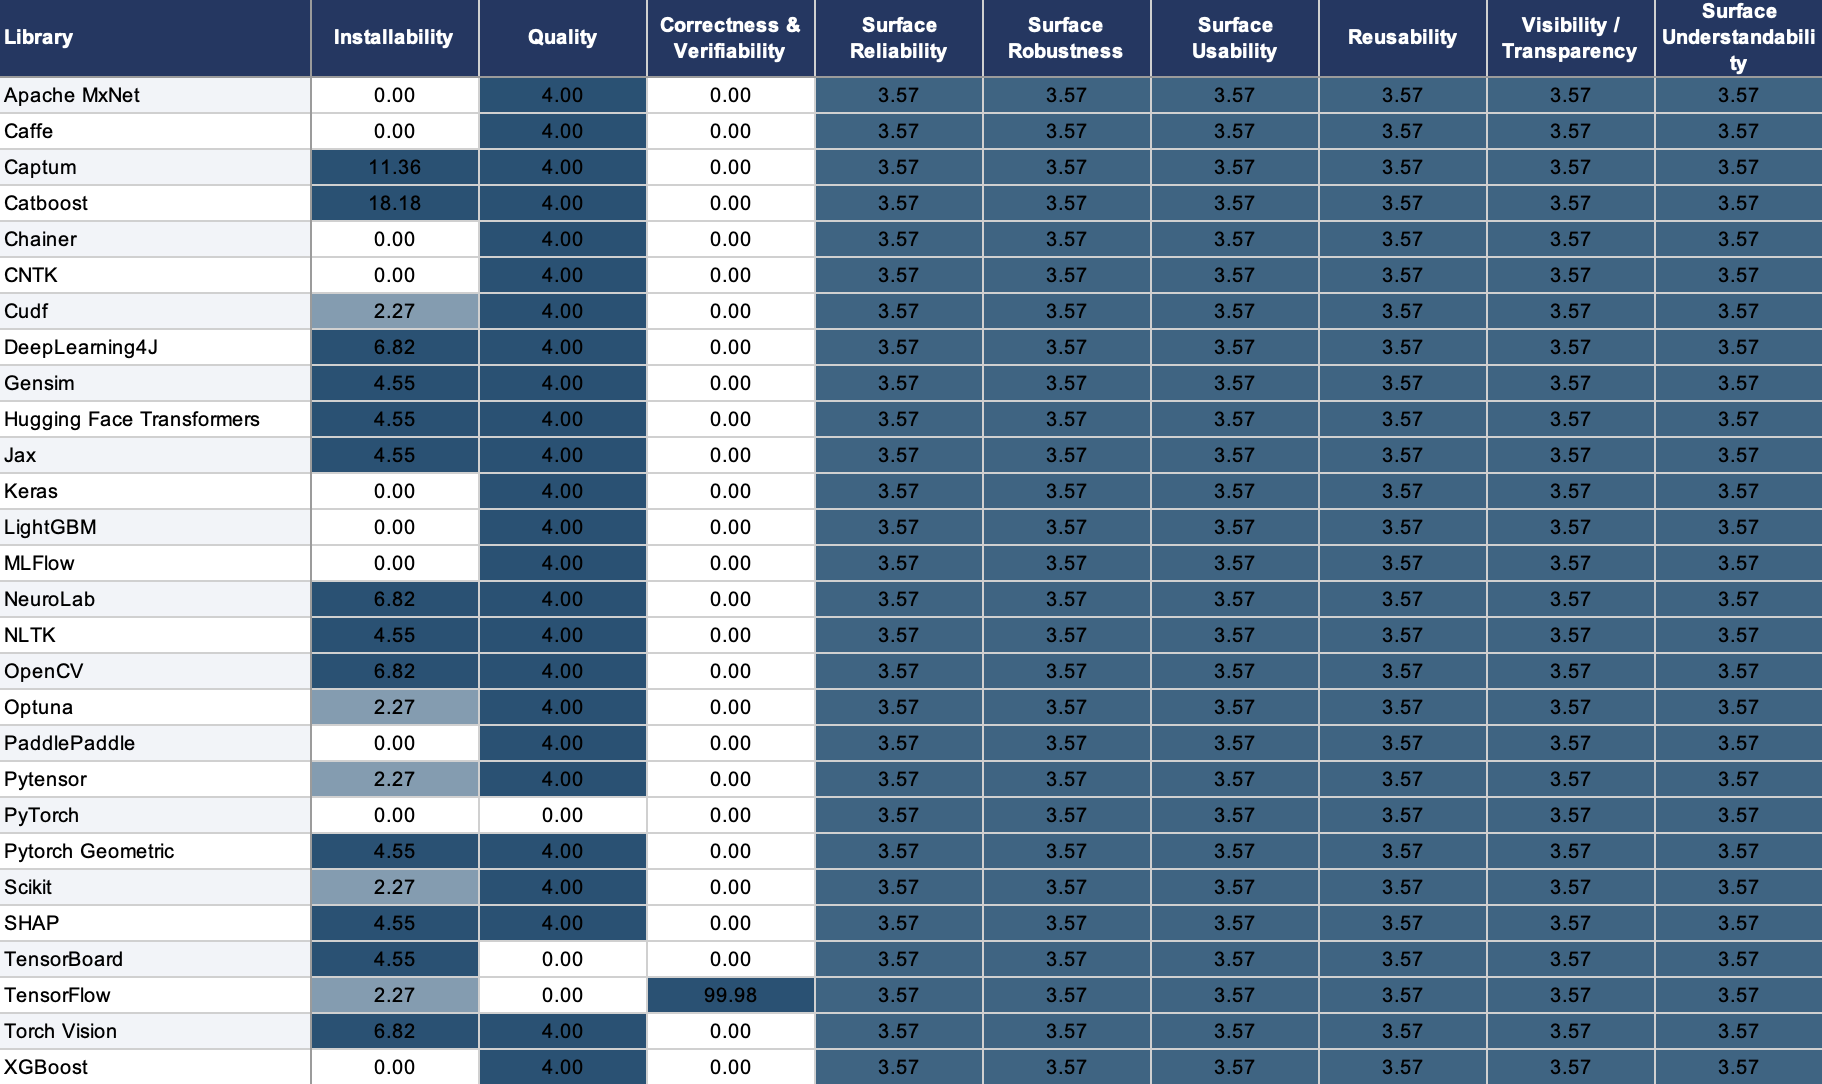
\includegraphics[width=\textwidth]{snapshots/nn_quality_heatmap.png}
  \caption{Heatmap summarizing per-quality scores for the
  28 shortlisted neural network software packages. Darker
  cells indicate larger values within a given category.}
  \label{fig:quality-heatmap}
\end{figure}

\subsection{Sensitivity analysis}\label{results-sensitivity}
\wss{ how rankings change under weight variation, identify stable vs unstable parts of the ranking and summary of implications.}

\subsection{Popularity vs evidence-based ranking (optional)}\label{results-popularity}
\wss{Compare evidence-based results against reputation indicators (e.g. stars/download). Discuss alignment/misalignment
 and what it suggests about state-of-practice versus  popularity.}

%%%%%%%%%%%%%%%%%%%%%%%%%%%%%%%%%%%%%%
%%%%%%%%%%%%%%%%%%%%%%%%%%%%%%%%%%%%%%
\section{Discussion and Recommendations}\label{discussion}
%%%%%%%%%%%%%%%%%%%%%%%%%%%%%%%%%%%%%%
%%%%%%%%%%%%%%%%%%%%%%%%%%%%%%%%%%%%%%
\wss{ what the results imply for users and maintainers. 
 actionable recommendations organized by quality attribute (installability, maintainability, transparency...). 
 Keep recommendations evidence-backed.}

%%%%%%%%%%%%%%%%%%%%%%%%%%%%%%%%%%%%%%
%%%%%%%%%%%%%%%%%%%%%%%%%%%%%%%%%%%%%%
\section{Threats to Validity and Limitations}\label{validity}
%%%%%%%%%%%%%%%%%%%%%%%%%%%%%%%%%%%%%%
%%%%%%%%%%%%%%%%%%%%%%%%%%%%%%%%%%%%%%
\wss{ construct validity, internal validity, external validity, and temporal validity. 
Note limitations such as evolving repositories, subjectivity in scoring, missing/ambiguous evidence,
 and interviews not conducted yet.}

%%%%%%%%%%%%%%%%%%%%%%%%%%%%%%%%%%%%%%
%%%%%%%%%%%%%%%%%%%%%%%%%%%%%%%%%%%%%%
\section{Conclusion and Future Work}\label{conclusion}
%%%%%%%%%%%%%%%%%%%%%%%%%%%%%%%%%%%%%%
%%%%%%%%%%%%%%%%%%%%%%%%%%%%%%%%%%%%%%
\wss{Summarize contributions (DomainX + dataset + findings), key results,  list future work 
(interviews, expanded shortlist, stronger sensitivity analysis, refined scoring rules, deeper automation).}

%%%%%%%%%%%%%%%%%%%%%%%%%%%%%%%%%%%%%%
%%%%%%%%%%%%%%%%%%%%%%%%%%%%%%%%%%%%%%
\appendix
%%%%%%%%%%%%%%%%%%%%%%%%%%%%%%%%%%%%%%
%%%%%%%%%%%%%%%%%%%%%%%%%%%%%%%%%%%%%%

\section{Assessed packages and exclusions}\label{app-packages}
\wss{table listing all assessed packages and excluded candidates with brief reasons to help traceability.}

\section{Measurement template excerpt and scoring rules}\label{app-template}
\wss{compact excerpt of measurement template and key scoring/normalization rules, or provide link to full template.}

\section{AHP weights and matrices}\label{app-ahp}
\wss{ final AHP weights and any matrices needed for transparency and reproducibility.}

\section{DomainX screenshots and exported artifacts}\label{app-tool}
\wss{potential figures: ranking view, table view, metric editing view, export example. }

%%%%%%%%%%%%%%%%%%%%%%%%%%%%%%%%%%%%%%
% References
%%%%%%%%%%%%%%%%%%%%%%%%%%%%%%%%%%%%%%
\bibliographystyle{plainnat}
\bibliography{../../refs/References}

\end{document}